%%% Template originaly created by Karol Kozioł (mail@karol-koziol.net) and modified for ShareLaTeX use

\documentclass[a4paper,11pt]{article}

\usepackage[T1]{fontenc}
\usepackage[utf8]{inputenc}
\usepackage{graphicx}
\usepackage{xcolor}
\usepackage{tgtermes}
\usepackage{listings}

\usepackage[
pdftitle={CSE258 Homework 1}, 
pdfauthor={Chenyu Huang, University of California San Diego},
colorlinks=true,linkcolor=blue,urlcolor=blue,citecolor=blue,bookmarks=true,
bookmarksopenlevel=2]{hyperref}
\usepackage{amsmath,amssymb,amsthm,textcomp}
\usepackage{enumerate}
\usepackage{multicol}
\usepackage{tikz}

\usepackage{geometry}
\geometry{total={210mm,297mm},
left=25mm,right=25mm,%
bindingoffset=0mm, top=20mm,bottom=20mm}


\linespread{1.3}

\newcommand{\linia}{\rule{\linewidth}{0.5pt}}

% custom theorems if needed
\newtheoremstyle{mytheor}
    {1ex}{1ex}{\normalfont}{0pt}{\scshape}{.}{1ex}
    {{\thmname{#1 }}{\thmnumber{#2}}{\thmnote{ (#3)}}}

\theoremstyle{mytheor}
\newtheorem{defi}{Definition}

% my own titles
\makeatletter
\renewcommand{\maketitle}{
\begin{center}
\vspace{2ex}
{\huge \textsc{\@title}}
\vspace{1ex}
\\
\linia\\
\@author \hfill \@date
\vspace{4ex}
\end{center}
}
\makeatother
%%%

% custom footers and headers
\usepackage{fancyhdr,lastpage}
\pagestyle{fancy}
\lhead{}
\chead{}
\rhead{}
\lfoot{Homework \textnumero{} 4}
\cfoot{}
\rfoot{Page \thepage\ /\ \pageref*{LastPage}}
\renewcommand{\headrulewidth}{0pt}
\renewcommand{\footrulewidth}{0pt}
%

% custom style for code
\lstdefinestyle{customc}{
  belowcaptionskip=1\baselineskip,
  breaklines=true,
  frame=L,
  xleftmargin=\parindent,
  language=C,
  showstringspaces=false,
  basicstyle=\footnotesize\ttfamily,
  keywordstyle=\bfseries\color{green!40!black},
  commentstyle=\itshape\color{purple!40!black},
  identifierstyle=\color{blue},
  stringstyle=\color{orange},
}

\lstdefinestyle{customasm}{
  belowcaptionskip=1\baselineskip,
  frame=L,
  xleftmargin=\parindent,
  language=[x86masm]Assembler,
  basicstyle=\footnotesize\ttfamily,
  commentstyle=\itshape\color{purple!40!black},
}

\lstset{escapechar=@,style=customc}

%%%----------%%%----------%%%----------%%%----------%%%

\begin{document}

\title{CSE258 Homework 4}

\author{Chenyu Huang, University of California San Diego}

\date{03/05/2017}

\maketitle

\section{Homework 4}

\paragraph{Task 1}

The 5 most common bigrams in the first 5000 reviews are:

\begin{figure}[h]
    \centering
    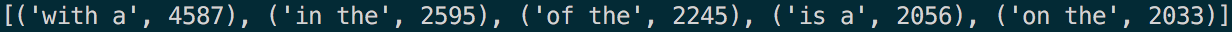
\includegraphics[width=16cm]{p1}
    \caption{5 most common bigrams}
\end{figure}
 
\paragraph{Task 2}

Using the most 1000 bigrams from the corpus, the MSE of the linear model is $0.343313$.

\paragraph{Task 3}

With a mixture of the most common bigrams and unigrams, the MSE of the model is $0.289394$.

\paragraph{Task 4}

The 5 words with the most common positive weights and 5 words with most negative weights are as follows:

Top 5 words with the most positive weights:

\begin{align}
('sort', 0.50408647668155093),\\ ('a bad', 0.22799617008799439), \\('of these', 0.22066627419916279), \\('not bad', 0.21355987652123357), \\('the best', 0.20916785548604572)
\end{align}

Top 5 words with the most negative weights:

\begin{align}
('straw', -0.19930067914769131), \\('the background', -0.22131852632951593), \\('corn', -0.23815182761392634), \\('water', -0.27289904891323319), \\('sort of', -0.63021419493511976)
 \end{align}

\clearpage

\paragraph{Task 5}

The IDF of the words are:
\begin{align}
('foam': 1.1139433523068367), \\('smell': 0.47712125471966244), \\('banana': 1.6720978579357175), \\('lactic': 2.9206450014067875), \\('tart': 1.806179973983887)
\end{align}

The TF-IDF of the words in the first review are:
\begin{align}
('foam': 2.2278867046136734), \\('smell': 0.47712125471966244), \\('banana': 3.344195715871435), \\('lactic': 5.841290002813575), \\('tart': 1.806179973983887)
\end{align}

\paragraph{Task 6}

Using just the 1000 most common unigram feature representation. The cosine similarity between the first and second reviews is: $0.106130241679$. 

\paragraph{Task 7}

Using only the 1000 most common unigram feature representation. The review with the highest cosine similarity with the first review has the following attributes:

\begin{align}
BeerId: 52211\\
Profile \ Name: Heatwave33
\end{align}

\paragraph{Task 8}
Using tf-idf as their feature representation, the MSE of the unigram model now is: $0.278742$


\clearpage

\section{Code}
\lstinputlisting[language=Python, caption={task1}]{p1.py}\clearpage
\lstinputlisting[language=Python, caption={task2}]{p2.py}\clearpage
\lstinputlisting[language=Python, caption={task3 and 4}]{p3.py}\clearpage
\lstinputlisting[language=Python, caption={task5}]{p5.py}\clearpage
\lstinputlisting[language=Python, caption={task6}]{p6.py}\clearpage
\lstinputlisting[language=Python, caption={task7}]{p7.py}\clearpage
\lstinputlisting[language=Python, caption={task8}]{p8.py}\clearpage


\end{document}
